% slides for neo-presention
\documentclass{beamer}

\usepackage[ngerman]{babel}
\usepackage[latin1]{inputenc}

\usetheme{Copenhagen}

\setbeamercovered{transparent}
\beamertemplatenavigationsymbolsempty
\setbeamertemplate{footline}[frame number]

\usecolortheme{seahorse}

\titlegraphic{
\includegraphics[width=4cm]{images/logo.png}}

\title{NEO - Ergonomisch optimiert}

\author[M. Schmidinger]{
    Markus Schmidinger
}

\begin{document}

\begin{frame}[plain]
  \titlepage
\end{frame}

\frame[plain]{
  \frametitle{Inhaltsverzeichnis}
  \tableofcontents
  [hideallsubsections]
}

%\begin{frame}[fragile]{NEO}{Ergonomisch optimiert}
%\end{frame}

\section{Ebenen}
\subsection{Ebene 1/2}
\frame[label=Ebene1_2]{
  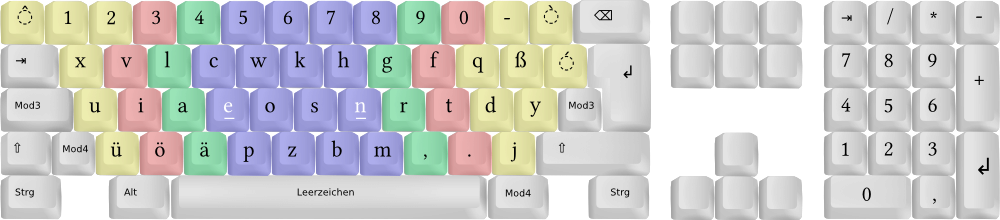
\includegraphics[width=\linewidth]{images/neo_ebene1.png}
}

\subsection{Ebene 3}
\frame[label=Ebene3]{
  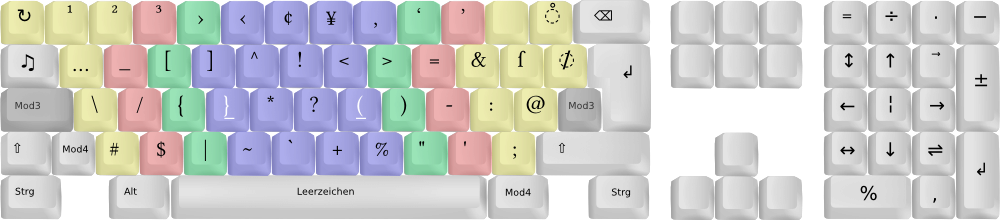
\includegraphics[width=\linewidth]{images/neo_ebene3.png}
}

\subsection{Ebene 4}
\frame[label=Ebene4]{
  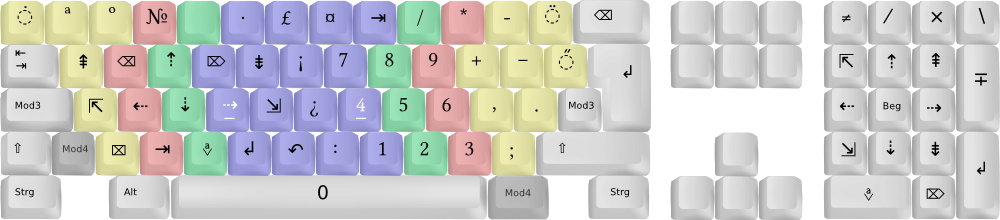
\includegraphics[width=\linewidth]{images/neo_ebene4.png}
}
  

%\frame[<+->][label=Liste]{
%  \frametitle{"Uberschrift}
%   \begin{itemize}
%     \item uno
%     \item duo
%   \end{itemize}
%}


\end{document}
